\documentclass{beamer}
\usepackage[spanish]{babel}
\selectlanguage{spanish}
\usepackage{graphicx}
\usepackage{float}
\usepackage{graphicx,subcaption}
\usepackage[utf8]{inputenc}
\usepackage[font=scriptsize,labelfont=bf]{caption}
\usepackage{ragged2e}
\usepackage{booktabs}
\usepackage{tikz}
\usepackage{listings}

\graphicspath{{/home/daniu/Documents/charla_GIS/figuras/}}

\AtBeginSection[]{
	\begin{frame}
		\vfill
		\centering
		\begin{beamercolorbox}[sep=8pt,center,shadow=true,rounded=true]{title}
			\usebeamerfont{title}\insertsectionhead\par%
		\end{beamercolorbox}
		\vfill
	\end{frame}
}
\usetheme{Madrid}

\title[Python para SIG]{Caracterización espacio-temporal de la clorofila en el mar argentino mediante herramientas de Python}
\subtitle{}
\author[Risaro, Daniela B]{Daniela B. Risaro\inst{1} \inst{2}}

\author[Risaro, Daniela B]{\parbox{.5\textwidth}{\centering {Daniela B. Risaro\inst{1} \inst{2}}\\[3pt]
		\scriptsize Twitter: \href{http://www.twitter.com/dbrisaro}{@dbrisaro} \\
		Github: \href{https://github.com/dbrisaro/charla_GIS}{Repositorio Github}}}

\institute[SHN-UBA] % (optional)
{
	\inst{1}%
	Departamento de Oceanografía\\
	Servicio de Hidrografía Naval (SHN)
	\and
	\inst{2}%
	Facultad de Cs Exactas y Naturales\\
	Universidad de Buenos Aires (UBA)
}
\date{\today}

\begin{document}
\begin{frame}
 \titlepage
\end{frame}

\begin{frame}
\frametitle{Esquema}
\tableofcontents
\end{frame} 

\section{Motivación}

\begin{frame}
 \frametitle{Area de estudio - El mar argentino}
 
\begin{figure}
 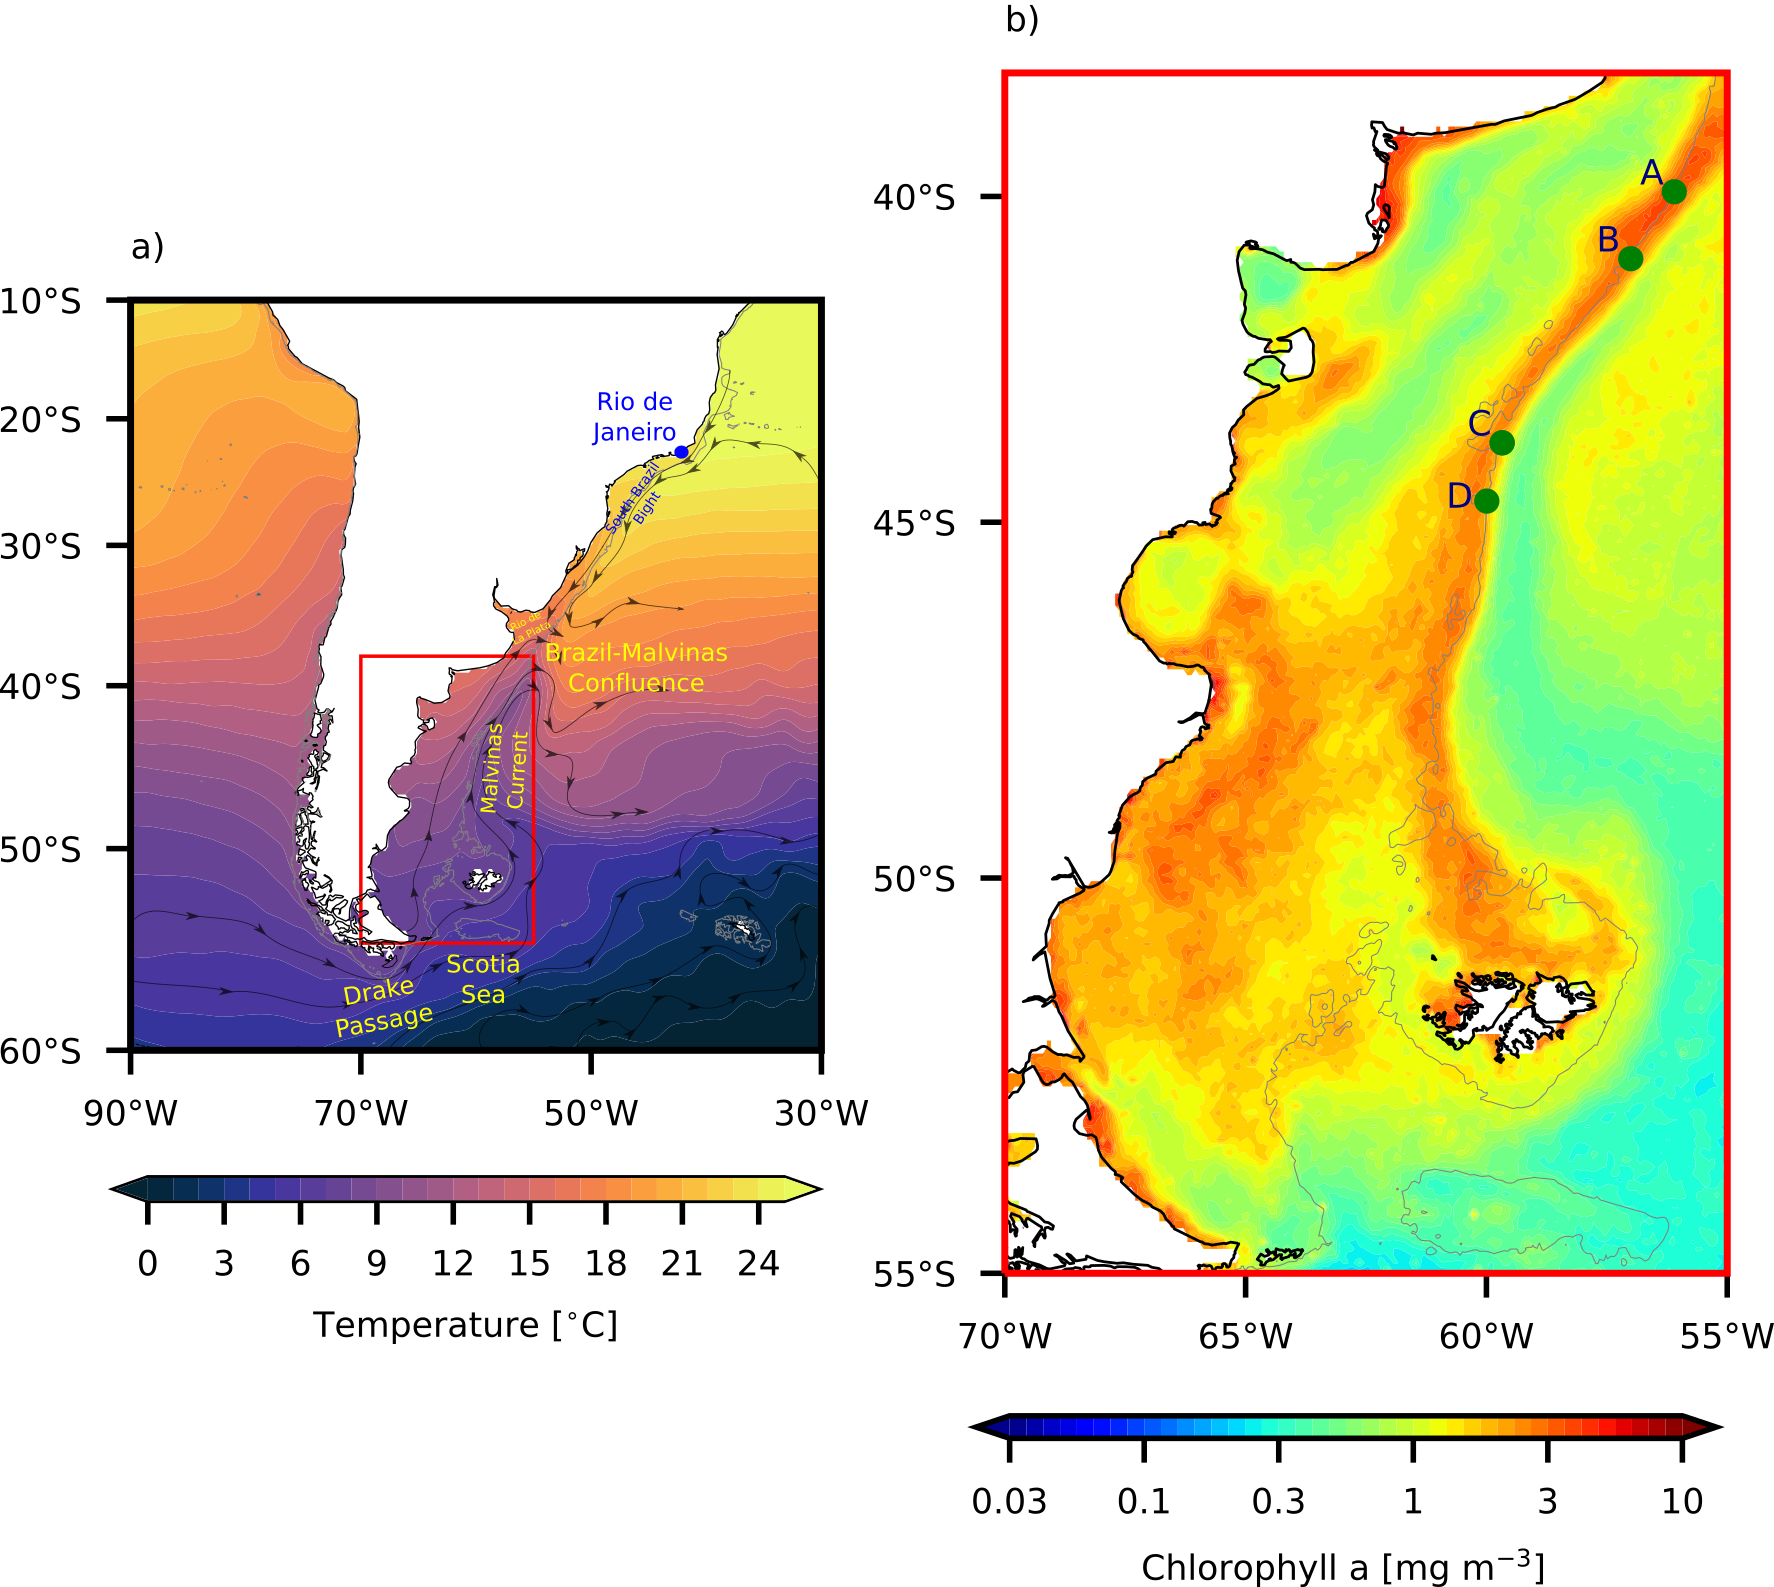
\includegraphics[scale=0.83]{intro.png}
\caption{a) Distribucion climatológica de TSM en el Atlántico Sudoccidental junto principales corrientes oceánicas. b) Clorofila superficial media durante la primavera en la plataforma patagónica.}
 \end{figure}
\end{frame}


\section{Datos de clorofila}

\begin{frame}[t]
 \frametitle{Datos disponibles - clorofila-a}

  \begin{itemize}
   \item<1-> Mediciones in-situ \pause $\rightarrow$ muy escasas
   \item<3-> Satelitales  \pause $\rightarrow$ sensores de color
      
   \begin{figure}
   	\begin{tikzpicture}
   	\node[anchor=south west,inner sep=0] at (0,0) {\includegraphics<4->[scale=0.9]{global_ocean_color_sensors.pdf}};
   	\draw<5->[red,thick,rounded corners] (3.55,2.1) rectangle (5.8,2.45);
   	\draw<6->[red,thick,rounded corners] (4.3 ,2.55) rectangle (7.7, 2.9);
   	\end{tikzpicture}	
   \end{figure}

\item[]<7->\tiny{Fuente: \href{https://oceancolor.gsfc.nasa.gov/docs/odps_opdsmp.may2018.pdf}{\beamergotobutton{Link}}}
  \end{itemize}
\end{frame}


\begin{frame}[t]
\frametitle{Archivos}

\begin{itemize}
	\item<1-> ¿Dónde encuentro esta información? $\rightarrow$ Ocean color \href{https://oceancolor.gsfc.nasa.gov/}{\beamergotobutton{Link}}

	\item<2-> Niveles de procesamiento:
\begin{itemize}
	\item L1 y L2
	\item L3 $\rightarrow$ grillados 
\end{itemize}

   \begin{figure}
	
	\begin{tikzpicture}
	\node[anchor=south west,inner sep=0] at (0,0) {\includegraphics<4->[scale=0.22]{L3browser.png}};
	\draw<5->[red,thick,rounded corners] (1.5, 2.7) rectangle (2.5, 2.9);
	\draw<6->[red,thick,rounded corners] (3.7, 2.7) rectangle (4.5, 2.9);
	\draw<7->[red,thick,rounded corners] (6.2, 2.7) rectangle (7, 2.9);
	\draw<8->[red,thick,rounded corners] (8.5, 2.7) rectangle (9.5, 2.9);
	\draw<9->[red,thick,rounded corners] (0.15, 2.3) rectangle (6, 2.5);
	\draw<10->[black,thick,rounded corners] (7.3, 3) rectangle (9.1, 3.4);			
	\end{tikzpicture}	
	
   \end{figure}

\end{itemize}
\end{frame}


\begin{frame}[fragile]
\frametitle{Archivos}

\begin{itemize}
	\item<1-> Luego de seleccionar la opcion 'Mapped' uno obtiene una lista de links de archivos netCDF (.nc)
	\item<2-> \url{https://oceandata.sci.gsfc.nasa.gov/cgi/getfile/A20022132002243.L3m_MO_CHL.x_chlor_a.nc} \href{https://oceandata.sci.gsfc.nasa.gov/cgi/getfile/A20022132002243.L3m_MO_CHL.x_chlor_a.nc}{\beamergotobutton{Link}}
\end{itemize}

\begin{itemize}
	\item[]<3-> Si son varios archivos:
	\item<4-> generar un archivo datos.txt 
	\item<4-> ejecutar en la terminal el comando 
	
	\begin{lstlisting}[language=bash, basicstyle=\scriptsize]
	cd /home/daniu/Documentos/charla_gis/
	wget -i datos.txt  
	\end{lstlisting}
\end{itemize}

\end{frame}


\begin{frame}[fragile]
\frametitle{Archivos}

\begin{itemize}
	
\item<1-> Un archivo netCDF (Network Common Data Form) es un formato que guarda datos multidimensionales para variables climáticas, por ejemplo:

\begin{itemize}
	
	\item<2-> TSM (tiempo, latitud, longitud)
	\item<2-> Taire (tiempo, latitud, longitud, presion)
	\item<2-> clorofila-a (tiempo, latitud, longitud)
	
\end{itemize}

\item<3-> El archivo .nc tiene un \textit{header} que contiene toda la información sobre las dimensiones y atributos de las variables, pero no los valores en si. Los datos están comprimidos en la \textit{data-part} del archivo. 

\end{itemize}

\end{frame}


\begin{frame}[fragile]
\frametitle{Archivos}

Para visualizar la información del \textit{header} podemos ejecutar en la terminal:

\begin{lstlisting}[language=bash, basicstyle=\scriptsize]
cd /home/daniu/charla_gis/
ncdump -h A20022132002243.L3m_MO_CHL.x_chlor_a.nc
\end{lstlisting}

y obtenemos lo siguiente:

\begin{figure}

\begin{tikzpicture}
   \node[anchor=south west,inner sep=0] at (0,0) {\includegraphics<1->[scale=0.2]{ncdump-console.png}};
   \draw<3->[->] (-0.9, 5.3) -- (-0.3, 5.3);
   \draw<4->[->] (-0.9, 4.7) -- (-0.3, 4.7);
   \draw<5->[->] (-0.9, 1.2) -- (-0.3, 1.2);      
\end{tikzpicture}

\end{figure}

\end{frame}

\section{Python workflow}

\begin{frame}[t,fragile]
\frametitle{Manipulación .nc en python}

\begin{itemize}

	\item<1-> En Python hay una libreria especializada en la manipulación de archivos netCDF llamada \texttt{xarray} (más info en: \href{http://xarray.pydata.org/en/stable/}{\beamergotobutton{Link}})

	\item[]<2-> 
	\begin{figure}
		\begin{tikzpicture}
		\node[anchor=south west,inner sep=0] at (0,0) {\includegraphics<3->[scale=0.15]{dataset-diagram.png}};
		\end{tikzpicture}
	\end{figure}

	\item[]<4-> 

\begin{lstlisting}[language=python, basicstyle=\scriptsize]
import xarray as xr

dire = '/home/daniu/Documentos/charla_gis/'
filename = 'A20022132002243.L3m_MO_CHL.x_chlor_a.nc'
data = xr.open_dataset(dire + filename)
print(data_chl)
\end{lstlisting}

\end{itemize}
\end{frame}


\begin{frame}[fragile]
\frametitle{Operaciones con xarray}

\begin{itemize}
	\item[]<1->
\begin{lstlisting}[language=python, basicstyle=\scriptsize]
import xarray as xr

dire = '/home/daniu/Documentos/charla_gis/'
filename = 'A20022132002243.L3m_MO_CHL.x_chlor_a.nc'
data_chl = xr.open_dataset(dire + filename)

print(data_chl)
\end{lstlisting}

	\item[]<2->
\begin{figure}
	
	\begin{tikzpicture}
	\node[anchor=south west,inner sep=0] at (0,0) {\includegraphics<1->[scale=0.3]{xarray-info.png}};
	\end{tikzpicture}
	
\end{figure}

\end{itemize}
\end{frame}


\begin{frame}[t,fragile]
\frametitle{Operaciones con xarray - Mapas}
\begin{itemize}
	\item[]<1->
\begin{lstlisting}[language=python, basicstyle=\scriptsize]
import xarray as xr

dire = '/home/daniu/Documentos/charla_gis/'
filename = 'A20022132002243.L3m_MO_CHL.x_chlor_a.nc'
data_chl = xr.open_dataset(dire + filename)
\end{lstlisting}
	\item[]<2->
\begin{lstlisting}[language=python, basicstyle=\scriptsize]
data_chl_pp = data_chl.sel(lat=slice(-40,-55), lon=slice(-70,-46))	# select an area
levels = np.linspace(0,3.5,15)
data_chl_pp.chlor_a.plot(levels=levels)					# simple plot
\end{lstlisting}
	\item[]<3->
\begin{figure}
	
	\begin{tikzpicture}
	\node[anchor=south west,inner sep=0] at (0,0) {\includegraphics<2->[scale=0.37]{map-chl.png}};
	\end{tikzpicture}
	
\end{figure}
\end{itemize}
\end{frame}

\begin{frame}[t, fragile]
\frametitle{Operaciones con xarray - Promedios espaciales}
\begin{itemize}
	
	\item[]<1->
\begin{lstlisting}[language=python, basicstyle=\scriptsize]
# zonal and meridional mean
mean_chl_zonal = data_chl_pp.mean(dim=('lon'))
mean_chl_meridional = data_chl_pp.mean(dim=('lat'))
\end{lstlisting}
	
	\item[]<2->
	\begin{lstlisting}[language=python, basicstyle=\scriptsize]
# plot of two panels
fig, ax = plt.subplots(1, 2)
mean_chl_zonal.chlor_a.plot(ax=ax[0])
mean_chl_meridional.chlor_a.plot(ax=ax[1])
	\end{lstlisting}
	
	\item[]<3->	
	\begin{figure}
		\begin{tikzpicture}
		\node[anchor=south west,inner sep=0] at (0,0) {\includegraphics<2->[scale=0.4]{zonal-merid-chl.pdf}};
		\end{tikzpicture}
	\end{figure}
	
\end{itemize}

\end{frame}

\begin{frame}[t, fragile]
\frametitle{Series temporales}

\begin{lstlisting}[language=python, basicstyle=\scriptsize]
# Load the file with the data of SWF and MODIS from 2000 to 2010
filename = 'chl_9km_70-55W_55-40S_2000-2010.nc'    
data_chl = xr.open_dataset(dire + filename)

data_chl_gsm = data_chl.sel(latitude=slice(-40, -43), 
			longitude=slice(-65, -60)) 

mean_chl_spatial = data_chl_gsm.mean(dim=('latitude', 'longitude'))

# plot of a mean time serie
mean_chl_spatial.chl.plot(aspect=3, size=2)
\end{lstlisting}

\begin{figure}
	
	\begin{tikzpicture}
	\node[anchor=south west,inner sep=0] at (0,0) {\includegraphics<2->[scale=0.6]{spatial-mean-timeseries-chl-gsm.pdf}};
	\end{tikzpicture}
	
\end{figure}

\end{frame}

\begin{frame}[t, fragile]
\frametitle{Series temporales}

\begin{lstlisting}[language=python, basicstyle=\scriptsize]

# plot of time series from selected gridpoints
data_chl_gsm_points = data_chl_gsm.sel(longitude=[-64], 
					latitude=[-42,-43], 
					method='nearest').squeeze()
data_chl_gsm_points.chl.plot.line(x='time', aspect=3, size=2)
\end{lstlisting}

\begin{figure}
	
	\begin{tikzpicture}
	\node[anchor=south west,inner sep=0] at (0,0) {\includegraphics<2->[scale=0.6]{gridpoints-timeseries-chl-gsm.pdf}};
	\end{tikzpicture}
	
\end{figure}

\end{frame}


\section{Resultados del mar Argentino}
\begin{frame}
	
\frametitle{Construccion series temporales}

\begin{itemize}
	\item<1-> Se realizo una serie que unifica a SWFs y MODIS en cada punto de grilla segun la metodología de \textit{Marrari et al 2015}
	\item<2-> SWF 1997-2010 
	\item<3-> MODIS 2002-presente
	\item[]<4-> $\rightarrow$ serie unica de clorofila desde 1997 hasta la actualidad con una resolucion espacial de 9km y datos diarios/semanales/mensuales
\end{itemize}

\end{frame}

\begin{frame}
	
\frametitle{Algunos plots}
\begin{figure}
	\begin{tikzpicture}
	\node[anchor=south west,inner sep=0] at (0,0) {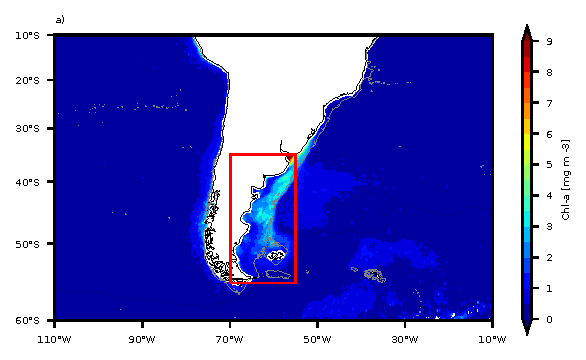
\includegraphics[scale=0.9]{media_spring_chl_a_1998-2017_swa_sep_25x25.pdf}};
	\end{tikzpicture}
	\caption{Distribucion climatológica de clorofila-a media durante los meses de primavera para el periodo 1998-2017}
\end{figure}
	
\end{frame}

\begin{frame}
	
	\frametitle{Algunos plots}
	\begin{figure}
		\begin{tikzpicture}
		\node[anchor=south west,inner sep=0] at (0,0) {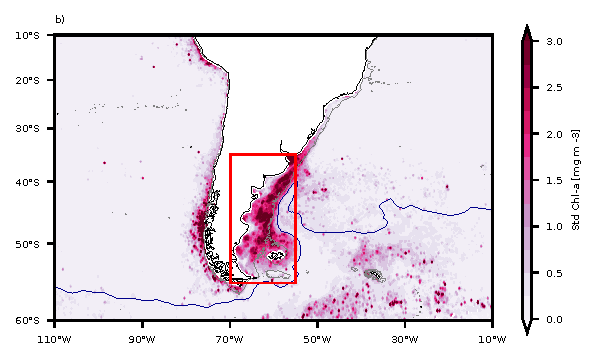
\includegraphics[scale=0.9]{std_spring_chl_a_1998-2017_swa_sep_25x25.pdf}};
		\end{tikzpicture}
	\caption{Distribucion del desvio estandar de clorofila-a durante los meses de primavera para el periodo 1998-2017}
	\end{figure}

\end{frame}

\begin{frame}
	
	\frametitle{Algunos plots}
	\begin{figure}
		\begin{tikzpicture}
		\node[anchor=south west,inner sep=0] at (0,0) {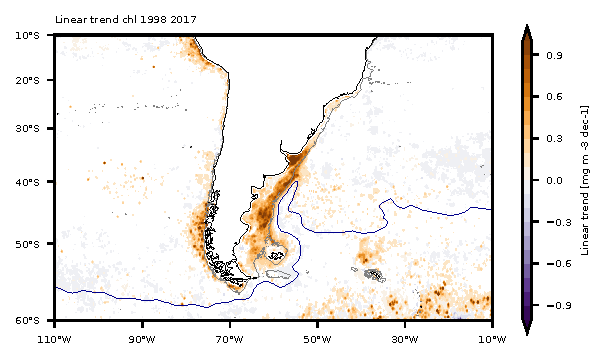
\includegraphics[scale=0.9]{trend_b_anom_chl_1998-2017_swa_sep.pdf}};
		\end{tikzpicture}
	\caption{Distribucion de tendencias lineales de anomalias de clorofila-a durante el periodo 1998-2017}	
	\end{figure}

\end{frame}

\begin{frame}
	
	\frametitle{Algunos plots}
	\begin{figure}
		\begin{tikzpicture}
		\node[anchor=south west,inner sep=0] at (0,0) {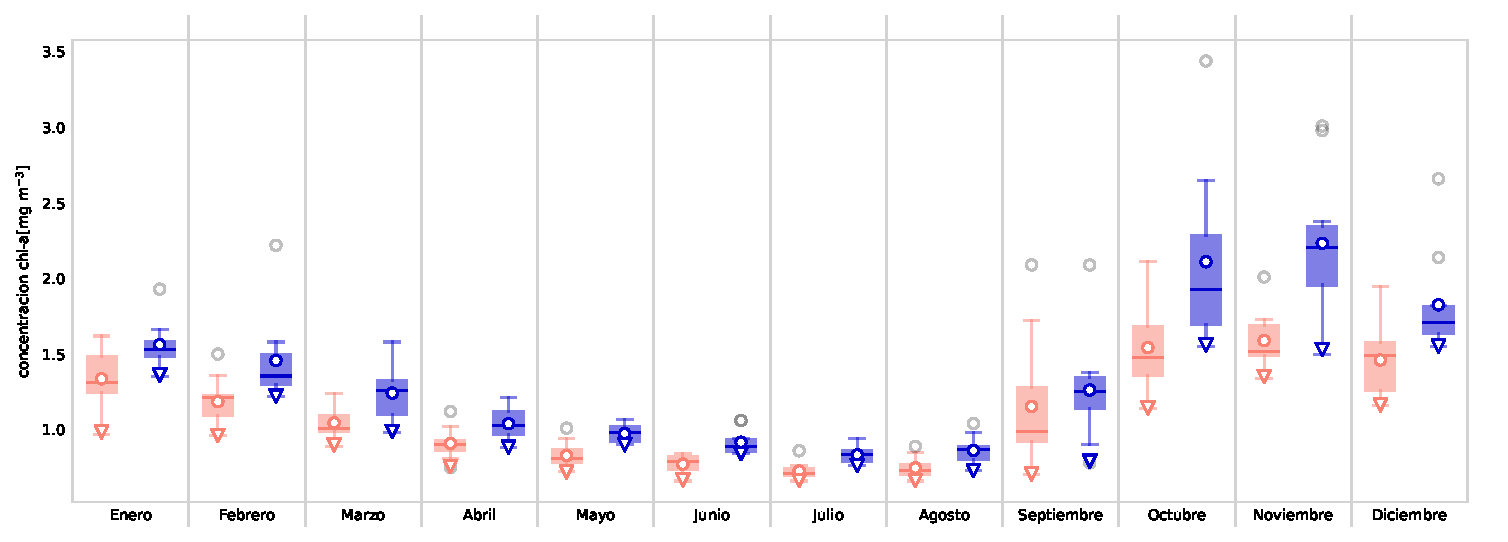
\includegraphics[scale=0.45]{whiskers_plot_chl_70-55W_55-35S.pdf}};
		\end{tikzpicture}
	\caption{Evolucion del ciclo climatologico de clorofila-a para los periodos 1998-2007 y 2008-2017}	
	\end{figure}
	
\end{frame}



\end{document}
